\section{Future Directions}

\begin{frame}{Performance vs. Number of Iterations}
    \textbf{Exploring Iterative Improvement:}
    \begin{itemize}
        \item In our current study, we conducted four types of experiments, each involving a single pass through 1000 problems due to cost constraints.

        \item Future research should investigate the relationship between performance and the number of maximum iterations.

        \item Understanding how performance scales with additional iterations could provide insights into the efficiency and effectiveness of iterative approaches.

        \item This could help in optimizing resource allocation for large-scale experiments and improving the overall performance of the CoT-SelfEvolve framework.
    \end{itemize}
\end{frame}

\begin{frame}{Using Metrics for Improvement}
    \begin{columns}
        \column{0.65\textwidth}
        \begin{itemize}
            \item \textbf{Current Limitation:} Each problem-solving attempt in CoT-SelfEvolve is treated as an independent instance.

            \item \textbf{Opportunity:} Leverage metadata (solution correctness, iterations, token cost) from these attempts.

            \item \textbf{Inspiration:} DSPy~\cite{khattab2023dspy} framework auto-optimizes prompts using:
                  \begin{enumerate}
                      \item Demonstrations based on labels and metrics.
                      \item Rewriting prompts and collecting metrics.
                  \end{enumerate}

            \item \textbf{Future Work:} Use collected metrics to select effective demonstrations for the Auto-CoT prompt generator.
        \end{itemize}

        \column{0.35\textwidth}
        \begin{figure}[H]
            \centering
            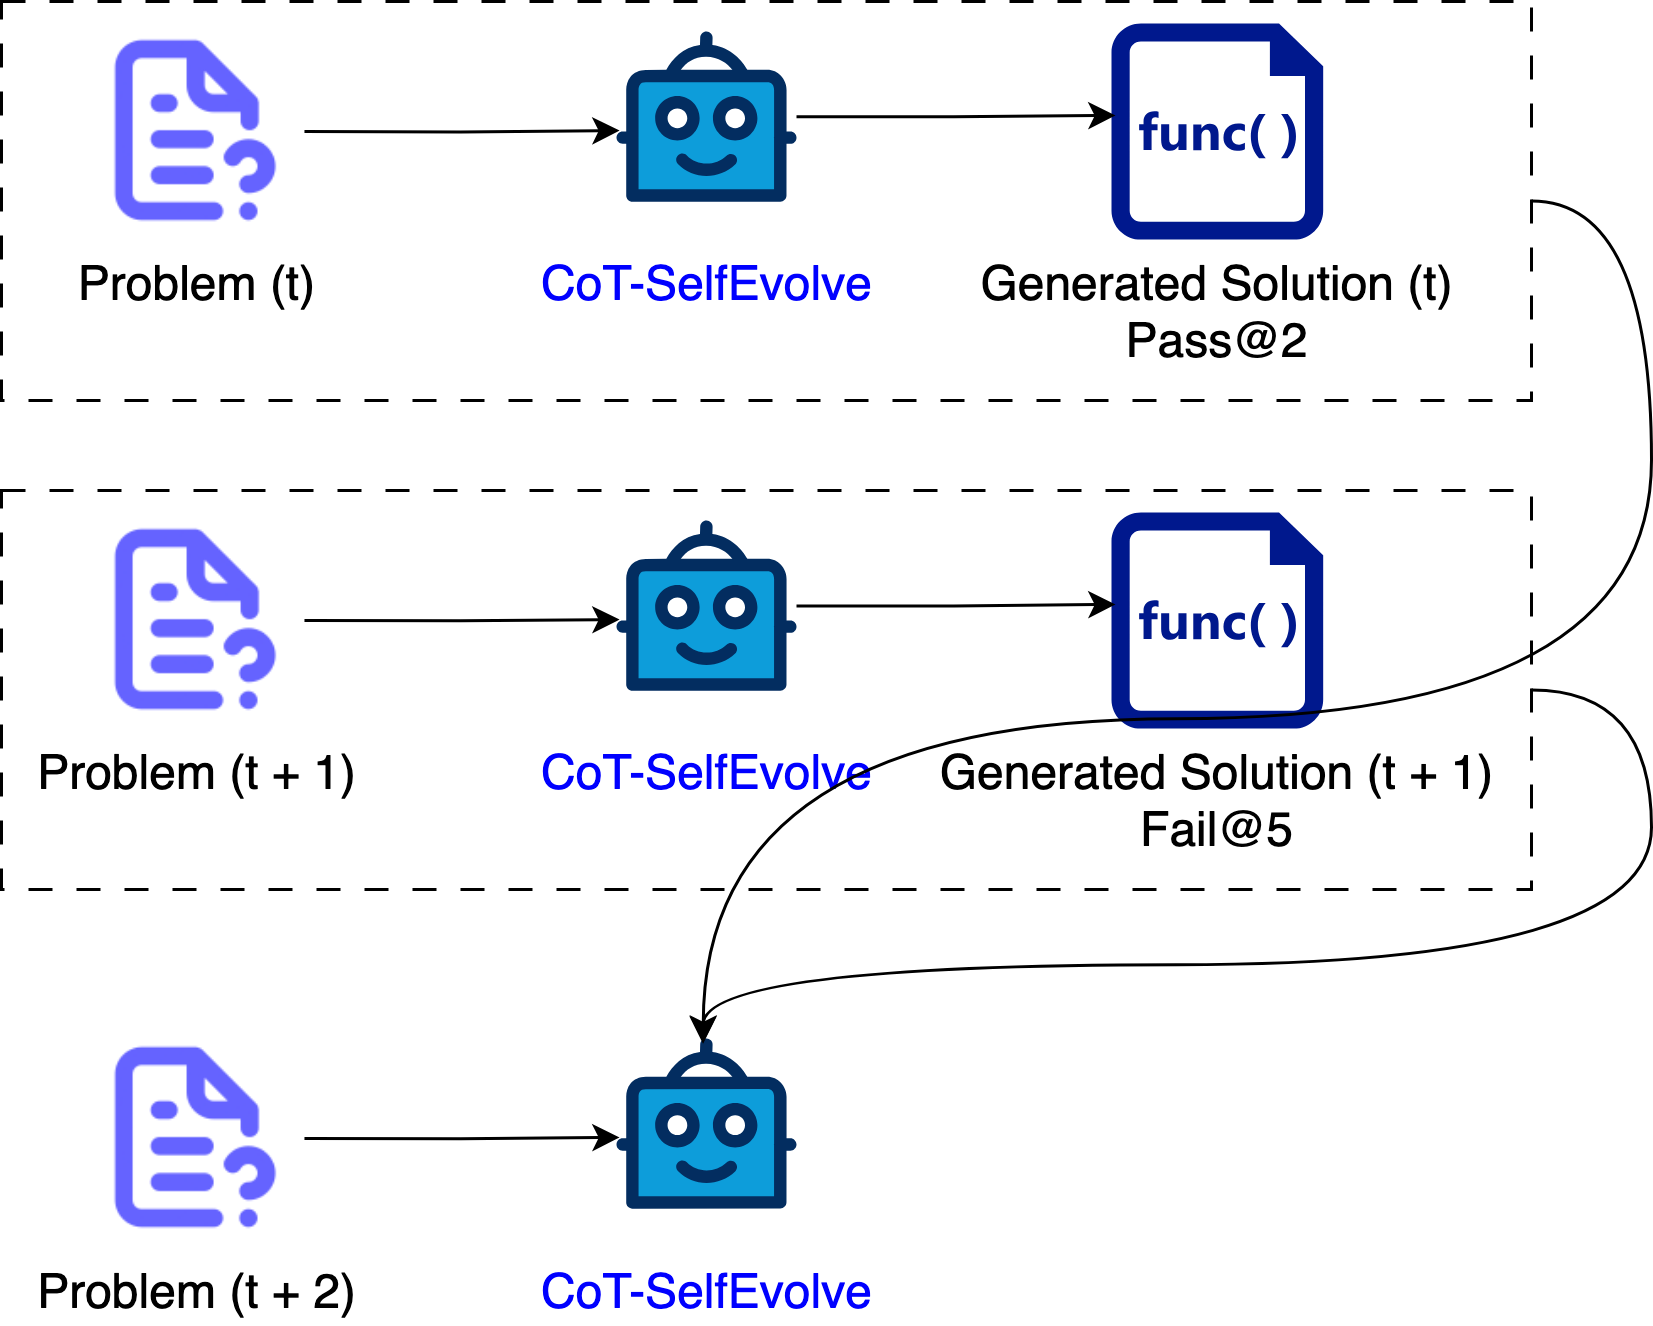
\includegraphics[width=\columnwidth]{img/enhanced_cot_selfevolve}
            \caption*{Leveraging metrics from prior runs to enhance CoT-SelfEvolve.}
        \end{figure}
    \end{columns}
\end{frame}
